\chapter{波动光学2(衍射)}
\section{选择题}
\exercise A

\solve
由于形成中央亮条纹的光是垂直通过单缝,在经过聚透镜后会聚焦到光轴上。所以聚透镜向y轴正方向平移,则中央衍射条纹会向上移动。又因为中央亮条纹宽度为$k=1$与$k=-1$两条暗条纹之间的距离。则有$bsin\varphi=\pm2k\frac{\lambda}{2},k=1$,当$b$减小,则$\varphi$增大,又因为$tan\varphi=\frac{x_1}{f}$,所以$x_1$增大,即中央亮条纹会变宽。

\exercise B

\solve
要让分辨本领大,则最小分辨角$\delta_\varphi$要尽量小,又因为$\delta_\varphi=\varphi_0\approx1.22\frac{\lambda}{D}$,电子波长比可见光波长小,即$\lambda$小,则电子波的$\delta_\varphi$更小,分辨率更高。

\exercise D

\solve
\begin{figure}[htbp]
\centering
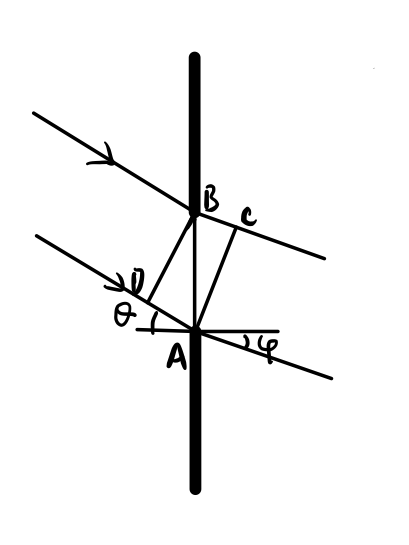
\includegraphics[width=0.30\linewidth]{Chp16_3.PNG}
\caption{题3 光路图}\label{fig:16_3}
\end{figure}
如图\ref{fig:16_3},光程差$\Delta=BC-DA=a(sin\phi-sin\theta)$;

中央亮条纹满足$a(sin\phi-sin\theta)=0$,即$\phi=\theta$;

所以中央亮条纹会偏移$\theta$,所以移动的距离x=$ftan\theta$。

\exercise D

\solve
在进行光学测量时,条纹越亮、越细、分得越开,测量越精确。光栅衍射具有这样的效果。

\exercise C

\solve
由光栅方程$(a+b)sin\varphi=\pm k\lambda$。由于衍射光线的原因,即$asin\varphi=\pm k'\lambda$,$k'=1,2,3...$时出现暗条纹,即$k=k'\frac{a+b}{a}$=2k'时,原应该有的亮条纹会由于衍射变为暗条纹。除了中央亮条纹外,一边会出现3条亮条纹,其中$k=1,2,3...,k'=1,2,3...$即$k=2$时会出现暗条纹,即$k=1$时出现第一条明纹,$k=3$时出现第二条明纹。所以选C。

\exercise C

\solve
惠更斯-菲涅尔原理指的是从同一波前上各点发出的次波是相干波,经过传播在空间某点相遇时叠加是相干叠加。这条定理也适用光的干涉。

\exercise D

\solve
由最小分辨角公式$\delta_\varphi=\varphi_0\approx1.22\frac{\lambda}{D}$,带入数值算得$\delta_\varphi=5.3\times10^{-7}rad$。

\exercise B

\solve
对于中央亮条纹,它是由各色光同时合成的,所以为白色。又由于由紫光到红光的波长逐渐增大,又$asin\varphi=\pm k\lambda$,对于同级亮纹,波长越大,衍射方向角($\varphi$)越大。又由于几何关系得衍射方向角越大,在屏幕上的亮条纹离中央亮条纹越远。

\exercise B

\solve
由最小分辨角公式$\varphi_0\approx1.22\frac{\lambda}{D}$得,$\varphi=2.33\times10^{-4}rad$,所以物品大小为$l=\varphi\cdot H=2.33\times10^{-4}\times300\times10^{3}m=67.1m$。

\exercise C

\solve
由衍射公式$asin\varphi=\pm k\lambda$,以及几何关系$sin\varphi\approx tan\varphi=\frac{x}{f}$,解得宽度$d=2x=\frac{2\lambda f}{a}$,所以焦距$f$增大,$d$也增大。

\section{填空题}
\exercise 中心

\solve
由于规定最小分辨角通常采取瑞利判据,即一个圆斑像中心刚好落在另一圆斑像的第一级暗环上。

\exercise $2\lambda$

\solve
根据单缝衍射条纹的暗纹条件,即$asin\varphi=\pm2k\cdot\frac{\lambda}{2}$,在第二个暗条纹时,$k=2$。所以光程差$asin\varphi=2\lambda$。

\exercise $6.04\times10^{-5}\mathrm{m}$

\solve
根据单缝衍射条纹的暗纹条件,即$asin\varphi=\pm2k\frac{\lambda}{2}$,对于第一级暗条纹,$k=1$。其中$\varphi=1.2°/2=0.6°$,代入方程得$a=\frac{\lambda}{sin\varphi}=\frac{632.8\times10^{-9}}{sin(0.6°)}m=6.04\times10^{-5}m$。

\exercise $1.2\times10^{-3}\mathrm{m}$\quad $3.6\times10^{-3}\mathrm{m}$

\solve
根据单缝衍射条纹的暗纹条件,即$bsin\varphi=\pm2k\frac{\lambda}{2}$,又由于几何关系$sin\varphi\approx tan\varphi=\frac{x}{f}$,得$d=2x=\frac{2k\lambda f}{a}$。 当计算中央明条纹宽度时,$k=1$,所以$d_1=\frac{2\times600\times10^{-9}\times60\times10^{-2}}{0.6\times10^{-3}}m=1.2\times10^{-3}\mathrm{m}$。对于两个第三级暗纹之间的距离,$k=3$,此时$d_3=\frac{6\times600\times10^{-9}\times60\times10^{-2}}{0.6\times10^{-3}}\mathrm{m}=3.6\times10^{-3}\mathrm{m}$。

\exercise $10\lambda$

\solve
当$k=2$时,两个相邻的缝之间光程差为$dsin\varphi=2\lambda$,第一条缝与第六条缝之间差5条缝,即光程差$\delta=5dsin\varphi=10\lambda$。

\exercise 500nm

\solve
根据单缝衍射条纹的暗纹条件,即$bsin\varphi=\pm2k\frac{\lambda}{2}$,又由于几何关系$sin\varphi\approx tan\varphi=\frac{x}{f}$,算得$\lambda=\frac{bx}{k\lambda}$。其中对于中央明条纹两侧的两个第三级暗纹,$k=3$,$2x=8\mathrm{mm}$,代入得$\lambda=\frac{0.15\times10^{-3}\times4\times10^{-3}}{3\times40\times10^{-2}}\mathrm{m}=500\times10^{-9}\mathrm{m}=500\mathrm{nm}$。

\exercise $\frac{\pi}{6}$

\solve
根据单缝衍射条纹的暗纹条件,即$asin\varphi=\pm2k\frac{\lambda}{2}$,中央亮条纹边缘即为第一级暗条纹,即$k=1$。又$a=2\lambda$,所以$\varphi=\frac{\pi}{6}$。

\exercise $2.68\times10^{-7}$

\solve
由最小分辨角公式$\delta_\varphi=\varphi_0\approx1.22\frac{\lambda}{D}$,代入数值算得$\delta_\varphi=2.68\times10^{-7}\mathrm{rad}$。

\exercise 4

\solve
根据单缝衍射条纹的暗纹条件,单缝宽$a=4\lambda$,得光程差为$asin\varphi=2\lambda$。所以该光程差可以分为$n=2\lambda\div\frac{\lambda}{2}=4$个半波带。

\exercise $2dsin\varphi=k\lambda,k=1,2,3...$

\solve
根据光波干涉加强的条件,即相干光波之间光程差相隔$k\lambda$,即$d(sin\theta+sin\theta)=k\lambda$,化简得$2dsin\varphi=k\lambda,k=1,2,3...$。
\begin{figure}[!h]
	\centering
	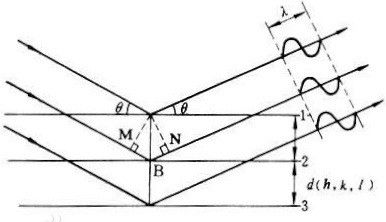
\includegraphics[width=0.5\linewidth]{Chp16_20.PNG}
	\caption{20题 光路图}
\end{figure}
\section{计算题}
\exercise

\solve
(1)由光栅方程$(a+b)sin\varphi=\pm k\lambda$;

当$\varphi=30°,k=1$时;

解得$a+b=10^{-6}\mathrm{m}$;

所以光栅常数为$10^{-6}\mathrm{m}$。

(2)由题意得:$\lambda=(1\pm5\% ) \lambda_0$;

代入光栅方程得:$(a+b)sin(\varphi\pm\frac{1}{2}\Delta\theta)=\pm k(1\pm5\%)\lambda_0$;

解得:$\theta_{min}=arcsin\frac{95\%\lambda_0}{a+b}=28.359°$;

$\theta_{max}=arcsin\frac{105\%\lambda_0}{a+b}=31.668°$;

得:$\Delta\theta\in[-1.641°,1.668°]$.

\exercise

\solve
根据单缝衍射条纹的暗纹条件,即$asin\varphi=\pm2k\frac{\lambda}{2}$;

中央亮纹的宽度为两侧第一级暗条纹的距离,此时$k=1$;

又由于几何关系:$sin\varphi\approx tan\varphi=\frac{x}{f}$;

当$2x=1.0\mathrm{cm}$时,$a_1=4.8\times10^{-5}\mathrm{m}$;
当$2x=1.5\mathrm{cm}$时,$a_2=3.2\times10^{-5}\mathrm{m}$;

即缝宽由$4.8\times10^{-5}\mathrm{m}$变为$3.2\times10^{-5}\mathrm{m}$。

\exercise

\solve
光栅衍射明条纹的条件为:$dsin\varphi=\pm2k\frac{\lambda}{2}$;

对光$\lambda_1$:$dsin\varphi=k_1\lambda_1$;

对光$\lambda_2$:$dsin\varphi=k_2\lambda_2$;

所以$k_1\lambda_1=k_2\lambda_2$,即$k_1=1.5k_2$;

当$k_1=3,k_2=2$时,两条光波第一次重合;

当$k_1'=6,k_2'=4$时,两条光波第二次重合

即$dsin\varphi=k_1'\lambda_1$;

得$d=\frac{k_1'\lambda_1}{sin\varphi}=3.05\times10^{-6}\mathrm{m}$。

\exercise

\solve
设最小分辨角为$\delta_\varphi$;

代入数据得:
\[
\delta_\varphi\approx\frac{1\mathrm{m}}{645\times10^{3}\mathrm{m}}=1.55\times10^{-6}\mathrm{rad}
\]
由最小分辨角公式$\delta_\varphi=\varphi_0\approx1.22\frac{\lambda}{D}$得:
\[
D=0.394\mathrm{m}
\]
